% !Mode:: "TeX:UTF-8"
\chapter{文献综述}

\section{研究现状}

\subsection{软件移植理论本身}

软件移植\upcite{krueger1992software}
指经过对原有软件的修改,是其运行在一个新的环境的过程,
该过程在软件工程理论中的软件生命周期中属于软件的维护阶段。
黄聪惠等学者\upcite{黄聪会2012软件移植理论与技术研究}指出软件移植
是一个使遗留系统适应新的软硬件环境的移动过程,要求软件的功能基本保持移植,
从而达到延长软件本身的生命周期的目的,而软件移植研究主要分为研究软件的可移植性理论和
研究软件移植的实现方法。将C++语言移植到html5/JavaScript语言属于
研究具体问题的的软件移植实现方法。

软件移植是软件重用的一种形式,通过与重用的比较,可以更深入的理解软件移植。
魏仁选等专家\upcite{魏仁选2002软件重用与移植的比较研究}总结了软件移植与软件重用的区别,
认为促进原有软件系统在新环境的重用是软件移植研究的目的,
重用是实现一个软件系统的软件制品在多种情形下的、广泛的重复使用。
而二者的区别在于移植实现在新平台和新环境下的运行,
而重用则着重于构建和维护软件构件集实现在新应用中的重复利用。因此,软件移植在研究目的和涉及的范围上都和软件重用不同。

软件的移植在不同的时期表现出了不同的特点\upcite{王建房2011从}。
早期的软件移植主要是解决软件移植到不同的体系结构和不同的操作系统,
以应对市场上的硬件和操作系统多样化、复杂化的特点,
基于图标、窗口、按钮和鼠标的图形用户界面问世后,软件移植转向CLI向GUI迁移。
Visual C++和Delphi的出现改善了开发环境,
软件移植的重点变为了保留结构化逻辑在图形界面下的实现,完成应用的代码移植。

软件移植主要分为\upcite{krueger1992software}源代码移植与二进制移植两种。
源代码移植通过修改与环境相关的部分源代码,是软件具备适应多种环境的能力;
二进制移植是指将软件从源环境移植到目标环境且能正确运行,
并与其在源环境下行为保持一致。
源代码移植方法的研究主要分为源代码移植的一般方法研究和具体移植问题的解决方法研究。

对源代码移植的一般方法研究有助于知道软件移植工作的展开。Fleuery\upcite{fleurey2007model}提出了使用模型驱动工程来进行源代码移植工作的方法。
他认为,遗留应用的移植需要有以下条件

\begin{itemize}
    \item 需求没有变化
    \item 移植到新的技术平台
    \item 设计上进行重构
\end{itemize}

他提出的模型驱动工程的方法如 图1-1 所示:

\begin{figure}[h!] % [h!] 表示尽量排在当前位置
    \centering
    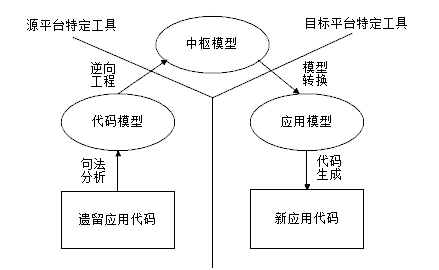
\includegraphics[width=200bp]{figure/pic/model-driving-software-porting.png}
    \caption{模型驱动工程的方法进行源代码移植}
    \label{model-driving-software-porting-sample}
\end{figure}

这一方法概述如下:首先对遗留应用的源代码进行句法分析,生成代码模型。
在完整了解遗留应用的前提下,通过对代码模型进行逆向工程,生成一个通用的中枢模型。
这一中枢模型具有可重用的特性,并且获取了索要移植的软件的全部信息,如:
静态结构,图形化用户界面,工作流(应用导航),方法和算法等。
接下来向目标环境进行模型转换,生成应用模型。
最后通过代码生成目标环境下对应的应用。

段成戈\upcite{段成戈2008基于重构偏序规划的软件移植方法研究}提出了采用基于偏序
规划的软件重构方法用于软件移植。该方法基于软件的结构变动信息,构建初始状态库和目标库,
对目标库建立重构的操作集,基于重构规划算法生成操作序列,按照操作序列完成软件的移植工作。

具体移植问题的解决方法研究可根据源和
目标环境分成不同类别\upcite{torchiano2008software}。
包括但不限于操作系统移植、数据库移植、编程语言移植、体系结构移植和用户界面移植。
C++到JavaScript属于编程语言移植。而桌面平台到web平台则同时属于操作系统移植、
编程语言移植、体系结构移植和用户界面移植。
皇甫俊彦\upcite{皇甫俊彦2011大型金融信息系统从}进行了从C\#到Java移植的研究,
提出了大型金融信息系统的源代码移植方案。其方法是分类方法,把软件讽刺XML界面文件,
数据库文件,逻辑代码等部分,然后针对不同的内容展开针对性的移植工作。
宋雨明\upcite{宋雨明2013iphone}进行了iOS平台到Android平台的软件移植工作的研究,
通过使用一系列的现有自动化工具,对逻辑代码、界面文件和资源文件进行针对性转换。

\subsection{llvm的优势}

对于普通的开发人员来说,LLVM计划\upcite{lattner2008llvm}提供了越来越多的可以使用、编译器以外的其他工具。例如代码静态检查工具 LLVM/Clang Static Analyzer,是一个 Clang 的子项目,能够使用同样的 Makefile 生成 HTML 格式的分析报告;而对关注编译技术的开发人员来说,LLVM提供了很多优点:现代化的设计:LLVM的设计是高度模块化的,使得其代码更为清晰和便于排查问题所在。语言无关的中间代码:这使得透过LLVM能够将不同的语言相互连结起来;另一方面,这也使得LLVM能够紧密地与IDE交互和集成。另一方面,发布中间代码而非目标代码能够在目标系统上更好地发挥其潜能而又不伤害可调试性(i.e. 在目标系统上针对本机的硬件环境产生目标代码,但又能够直接通过中间代码来进行行级调试)作为工具和函数库:使用LLVM提供的工具可以比较容易地实现新的编程语言的优化编译器或VM,或为现有的编程语言引入一些更好的优化\upcite{yermolovich2009optimization}/调试特性\upcite{lattner2008llvm}。

先来说说LLVM的历史。2000年LLVM开始开发,2005年Apple雇了Chris Lattner,LLVM也相当于成了Apple的官方支持的编译器。Apple已经将它用在OpenCL的流水线优化,Xcode已经能使用llvm-gcc编译代码。可以说05年之前LLVM一直都是学术界的东西,05年之后用于工业界.而这篇文章写在04年.本博最近听过一个关于LLVM的讨论会,会中有资深人士提到LLVM现在越来越像一个普通的编译器。说这番话的意思是,我们可以从这篇文章里找到LLVM的架构设计和早期的一些实现思想,但请不要迷信LLVM现在有多么神奇,每个架构都会有它的优缺点。

LLVM 是 Illinois 大学发起的一个开源项目,它到底是什么呢?从字面上看,它是一个虚机系统,然而这又和之前为大家所熟知的 JVM 以及 .net Runtime 这样的虚机不同,它提供了一套中立的中间代码和编译基础设施,并围绕这些设施提供了一套全新的编译策略(使得优化能够在编译、连接、运行环境执行过程中,以及安装之后以有效的方式进行)和其他一些非常有意思的功能。

对于普通的开发人员来说,LLVM计划提供了越来越多的可以使用、编译器以外的其他工具。例如代码静态检查工具 LLVM/Clang Static Analyzer,是一个 Clang 的子项目\upcite{clang2005language},能够使用同样的 Makefile 生成 HTML 格式的分析报告\upcite{jameson2006collection};而对关注编译技术的开发人员来说,LLVM提供了很多优点:

现代化的设计:LLVM的设计是高度模块化的,使得其代码更为清晰和便于排查问题所在。 语言无关的中间代码:这使得透过LLVM能够将不同的语言相互连结起来;而且,这也使得LLVM能够紧密地与IDE交互和集成。另一方面,发布中间代码而非目标代码能够在目标系统上更好地发挥其潜能而又不伤害可调试性(i.e. 在目标系统上针对本机的硬件环境产生目标代码,但又能够直接通过中间代码来进行行级调试) 作为工具和函数库:使用LLVM提供的工具可以比较容易地实现新的编程语言的优化编译器或VM,或为现有的编程语言引入一些更好的优化/调试特性。

\subsection{javascript target language的发展}

在ECMAScript 5.1 定稿之后,以JavaScript为编译目标的编程语言出现了很多,比如

\begin{enumerate}
    \item coffeescript\upcite{burnham2011coffeescript} 
    \item livescript\upcite{java1995netscape}
    \item typescript\upcite{hejlsberg2012introducing}
    \item clojurescript\upcite{mcgranaghan2011clojurescript}
    \item haXe\upcite{cannasse2008using}
\end{enumerate}

不过这些js target语言的出现不是为了软件移植,而是为了弥补JavaScript本身编写时的各种不足。

\subsection{传统软件向web移植的相关进展}

国内的开发者对于跨平台技术一直很热衷,
但是国内开发者研究的主题往往以 javascript 向安卓、ios 和桌面平台移植为主,
比如白鹭 egert 引擎和 cocos2d-js 引擎。
但鲜有对 C++向 javascript 的移植。
根据调研,仅有北京触控科技一家公司在产品 cocos2dx 2.x 的版本中,
使用了 emscripten 编译器将 C++ 代码编写的的游戏编译成 html5 版本;
在 cocos2dx 3.x 的版本中,将该功能移除。
推出了更适合 html5 开发者的 cocos2d-js。

国外企业和学者对于 C/S 软件向 B/S 移植则一直存在很大兴趣。

在互联网刚刚兴起时:

Microsoft 在传统软件移植 web 方面是研究比较早的。最出名的就是
Microsoft IE ActiveX 技术,该技术可以使用大量 win32 api,对于 windows 软
件移植代码量改动最小,几乎没有性能损失。但是需要安装插件,没认证过的插
件会被大多数安全软件拦截,并且只支持 windows 系统,不能应用于移动 web。
而且有很多安全问题。

Sun 公司和其后继者 Oracle 一直在持续改进 Java JNI \upcite{gordon1998essential} 技术。
该技术可以支持多种平台,浏览器兼容性好。但是操作系统跨平台需要额外工作,为每个平台
编译一个 Native 版本,需要目标平台安装 Java 且开启浏览器支持。

Adobe 公司为了方便传统软件向 flash 移植,开发了 flasCC 技术,该技术平
台兼容性比较好,而且 swf 文件可以脱离浏览器单独运行。但是目标机需要安装
flash player,移动设备现在大都不支持 flash player;而且渲染器需要重写,
3 维软件移植需要大量重写;价格高昂;编译过程非常缓慢。

Unity3D 公司也仿照 Adobe 公司的 flasCC 技术,推出了 unityWebPlayer 方
案,需要浏览器支持 PPAPI,但是只能移植 unity 平台开发的游戏,并且不支持
第三方插件,物理引擎和光照处理也不是很好。

在HTML5兴起之后

在 javascript 语言标准化制定完成(也即 ECMAscript 5.1 定稿)时,、,也恰逢
html5 技术兴起。

Google 为了方便 chrome web app 的开发,推出了 Google Native Client 技
术,简称 Google NaCl\upcite{metz2011google}。
NaCl 与 Native 性能差距不大,平台兼容性好。但是只支
持 chrome 浏览器 ,而且是 chrome web 应用,而不是网页。

Leaning Technologies 公司推出了 C++向 Javascript 编译器 Duetto,既可
以将 C++代码用于 web 应用的生成,也可以通过生成 node.js 脚本用于后端开发,
生成的 javascript 代码可以充分利用 javascript 的 JIT,性能较高。但是使用
LGPL 协议发布,商业不友好,开发完成程度不高,文档亦不够完善。

Mozilla 公司和 Epic 公司为了将 unreal engine runtime 移植到 web 上,开
发了基于 llvm+clang 的 C++ to Javascript 编译器, Emscripten\upcite{zakai2011emscripten},
可以使用 c++全部特性;依靠 asm.js \upcite{herman2013asm}解释器,将 javascript 直接解释为汇编代码运行,个别
测试效率超越 C++;支持 openGL ES 2.0 程序直接转变为 webGL \upcite{webgl20142}程序 。

Unity 公司在 2014 年开始 webGL 移植的实验。并使用 IL2CPP 技术和 Emscripten 编译器,将 C\#代码转换为 C++代码,再将 C++代码转换成 javascript 代码。使游戏移植到 webGL 上。并在 2015 年发布的 unity5.3 版本中,宣布 unity3D 已经完美支持 webGL 平台。

\section{实践意义}

软件移植使就有软件升入新的、更高更宽松的环境中,功能得以提高,应用范围得以扩大。将旧有软件直接移植到web,可以节约大量人力物力,更好的迎接互联网浪潮的来袭。